\documentclass[12pt,letterpaper,fleqn]{article}

%       amslatex provides nice math extensions for typesetting mathematics
\usepackage{amsmath}
\usepackage{amsfonts}
\usepackage{tmmaths}
\usepackage{sympytex}

%       pstricks provides powerful environments for incorporating postscript into a
%       TeX/LaTeX document. You must have a postscript printer and a package like
%       dvips to convert the DVI file to a PS file.
%\usepackage{pst-all}
%\usepackage{pstricks,pst-plot}
%\usepackage{pst-coil,pst-node}

%  This package provides native tex support for numbered grids. The syntax is:
%  \graphpaper[spc](x_lowleft,y_lowleft)(x_upperright,y_upperright)

%\usepackage{graphpap}
%\usepackage{float}

%  The package below must be initialized with "\initfloatingfigs" immediately after the
%  "\begin{document} command.
%\usepackage{floatfig}

\usepackage{graphicx}
\graphicspath{{i:/mytex/graphics}}
\DeclareGraphicsExtensions{.ps,.eps}

%       tst is a package for the creation of exams, quizzes and tests. the include
%       file mathstuf (see below) provides many abbreviations for these environments.
%\usepackage{tst}

%       epsfig is a package which provides for the inclusion of Encapsulated PostScript
%       files in a document.
%\usepackage{epsfig}
%\usepackage{epic,eepic}
\include{mathstuf}
\usepackage[total={7.25in,10in},top=0.25in,left=0.75in,includehead]{geometry}
\usepackage{fancyhdr}
\pagestyle{fancy}
\lhead{Math 252}
\rhead{\large Name\makebox[2in]{\hrulefill}}
\chead{\LARGE Exploration 15}
%\lfoot{\today}
\cfoot{}
%\rfoot{\thepage}
\renewcommand{\headrulewidth}{0.4pt}
\renewcommand{\footrulewidth}{0.4pt}
\setlength{\parindent}{0pt}
\setlength{\parskip}{2ex}

\newcounter{tf}[enumi]
\newenvironment{tf}[0]{\begin{list}%
{\alph{tf}. \makebox[5em]{True\hfill False}}%
{\usecounter{tf}\setlength{\labelwidth}{7em}%
\setlength{\leftmargin}{3.5cm}%
\setlength{\labelsep}{1cm}}}%
{\end{list}}

%\usepackage{epic,eepic}
\newcommand{\numline}{%
%\newcounter{mark}%
%\setcounter{mark}{-1}%
\setlength{\unitlength}{0.1in}%
\begin{picture}(0,0)%
\thicklines%
\put(0,0){\line(1,0){60}}%
\multiput(0,0)(10,0){7}{\line(0,-1){1}%
\makebox(0,-1.5)[t]{\arabic{mark}}\stepcounter{mark}}%
%
\thinlines%
\multiput(0,0)(5,0){12}{\line(0,-1){0.5}}%
\multiput(0,0)(1,0){60}{\line(0,-1){0.3}}%
%\put(-5,265){\makebox(0,0)[l]{{\bf cm}}}%
\end{picture}}%

\newcommand{\ds}{\displaystyle}
\usepackage{amsfonts}


\let\oldhat\hat
\renewcommand{\hat}[1]{\oldhat{\boldsymbol{\mathbf{#1}}}}
\newcommand{\lv}[1]{\ensuremath{\langle #1 \rangle}}
\renewcommand{\i}{\ensuremath{\hat{\imath}}}
\renewcommand{\j}{\ensuremath{\hat{\jmath}}}
\renewcommand{\k}{\ensuremath{\mathbf{\oldhat{k}}}}
\newcommand{\ora}[1]{\ensuremath{\overrightarrow{#1}}}
\renewcommand{\vec}[1]{\ensuremath{\mathbf{#1}}}
\renewcommand{\v}[1]{\ensuremath{\vec{#1}}}
\newcommand{\abs}[1]{\ensuremath{\lvert #1 \rvert}}

\usepackage{tabularx}
\usepackage{paralist}
\newcommand{\red}[1]{\textcolor{red}{#1}}
\newcommand{\blue}[1]{\textcolor{blue}{#1}}
% \newcommand{\ans}[1]{\quad\fbox{answer: \red{#1}}}
\newcommand{\ans}[1]{\mbox{{\bf Ans:} \blue{#1}}}
\newcommand{\dd}[2][]{\ensuremath{\frac{\text{d}#1}{\text{d}#2}}}
\newcommand{\eval}[2]{\ensuremath{\left.#1\right|_{#2}}}

\usepackage{amsthm}

\theoremstyle{definition}
\newtheorem*{definition}{Definition}

\usepackage{enumitem}
\usepackage{subfig}

\begin{document}
\section*{Trigonometric Substitution}
In this exploration we consider integrals whose integrands contain expressions of the form $a^2 - x^2$, $x^2 - a^2$ or $x^2 + a^2$ (especially when these expressions are under a square root), where $a$ is a constant. We will see that these integrands can sometimes be simplified by substituting various trigonometric functions for the $x$ variable in these expressions.\\[1.5ex] The trig.\ functions useful for this purpose are:
\begin{itemize}
 \item $a\sin\theta$
 \item $a\sec\theta$
 \item $a\tan\theta$
\end{itemize}
We will also need use of the trig.\ identities:
\begin{itemize}
 \item $1 - \sin^2\theta = \cos^2\theta$
 \item $1 + \tan^2\theta = \sec^2\theta$
\end{itemize}
\subsection*{Integrand contains $\pmb{a^2 - x^2}$}
Consider the integral $\int\sqrt{25 - x^2}\;dx$. Make the substitution $x = 5\sin\theta$ in the integral (don't forget to also substitute out the differential $dx$). You should now be able to simplify the resulting expression under the radical using one of the trig.\ identities above and end up with a radical free integrand. Complete the integration, to get an antiderivative in terms of the variable $\theta$.\\[1.5ex] Our final step is to get our $\theta$-antiderivative back to the original $x$ variable. The connection between these two variables is our original substitution $x = 5\sin\theta$. From this equation we can solve for $\theta$ in terms of $x$ and we can get any of the trig.\ functions of $\theta$ in terms of $x$.\\[1.5ex] Solving for $\theta$ gives $\theta = \arcsin(x/5)$. Solving for $\sin\theta$, we get $\sin\theta = \frac{x}{5}$. We can use this trig.\ relation between $x$ and $\theta$ to draw a right angled triangle (see the figure below) and use it to find any of the other trig.\ functions of $\theta$ in terms of $x$ and use these to get our antiderivative expression in terms of $x$.
\begin{figure}[!htb]
	\centering
	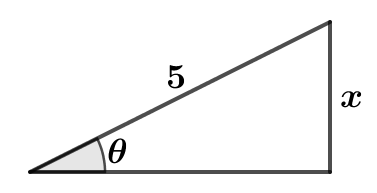
\includegraphics[width=2in]{img/trig_triangle.png}
	% \caption{}
	% \label{}
\end{figure}
Carrying out the above process, you should end up with:
\begin{equation*}
  \int\sqrt{25 - x^2}\;dx = \frac{25}{2}\arcsin\left(\frac{x}{5}\right) + \frac{x\sqrt{25-x^2}}{2} + C
\end{equation*}
\newpage
\section*{Integrand contains $\pmb{x^2 + a^2}$}
Consider the integral $\int\sqrt{x^2 + 25}\;dx$. Make the substitution $x = 5\tan\theta$ in the integral (don't forget to also substitute out the differential $dx$). Carry out a process similar to the one above to resolve the integral. Hint: $\int\sec^3\theta\;d\theta = \frac{1}{2}\sec\theta \tan\theta + \frac{1}{2}\ln|\sec\theta + \tan\theta|$\\[1.5ex] You should get:
\begin{equation*}
  \int\sqrt{x^2 + 25}\;dx = \frac{25}{2}\left[\frac{x\sqrt{x^2+25}}{25} + \ln\left|\frac{x + \sqrt{x^2+25}}{5}\right|\right] + C
\end{equation*}
\section*{Integrand contains $\pmb{x^2 - a^2}$}
Consider the integral $\int\sqrt{x^2 - 25}\;dx$. Make the substitution $x = 5\sec\theta$ in the integral (don't forget to also substitute out the differential $dx$). Carry out a process similar to the one above to resolve the integral. Hint: $\int\sec^3\theta\;d\theta = \frac{1}{2}\sec\theta \tan\theta + \frac{1}{2}\ln|\sec\theta + \tan\theta|$\\[1.5ex] You should get:
\begin{equation*}
  \int\sqrt{x^2 - 25}\;dx = \frac{25}{2}\left[\frac{x\sqrt{x^2-25}}{25} - \ln\left|\frac{x + \sqrt{x^2-25}}{5}\right|\right] + C
\end{equation*}
\end{document}
